\section*{Introduction}

\newenvironment{elaboration}{
\par
\begin{tikzpicture}
\node[rectangle,minimum width=\textwidth] (m)
\bgroup
\begin{minipage}{0.97\textwidth}}
{\end{minipage}\egroup;
\draw[dashed] (m.south west) rectangle (m.north east);
\end{tikzpicture}
}


Iliano is writing a new programming assignment called sets, where he
has students represent sets of integers as \lstinline'int' arrays. One
of the functions he wants them to write is \lstinline'intersect' which
computes the intersection of two arrays.  The relevant section of the
writeup is below:
\begin{elaboration}
\begin{lstlisting}[aboveskip=0pt]
int intersect(int[] A, int n, int[] B, int m, int[] intersection)
//@requires 0 <= n && n <= \length(A);
//@requires 0 <= m && m <= \length(B);
//@requires n <= \length(intersection) || m <= \length(intersection);
/*@ensures 0 <= \result && \result <= m && \result <= n; @*/ ;
\end{lstlisting}
The function \lstinline'intersect' computes the \emph{intersection} of
two arrays \lstinline'A' and \lstinline'B', defined as the array
containing all the elements that occur in both \lstinline'A' and
\lstinline'B' (in sorted order and without duplicates).  We do
\textbf{not} enforce that \lstinline'A' and \lstinline'B' have no
duplicates nor that they be sorted.  Here's an example:
\begin{center}
  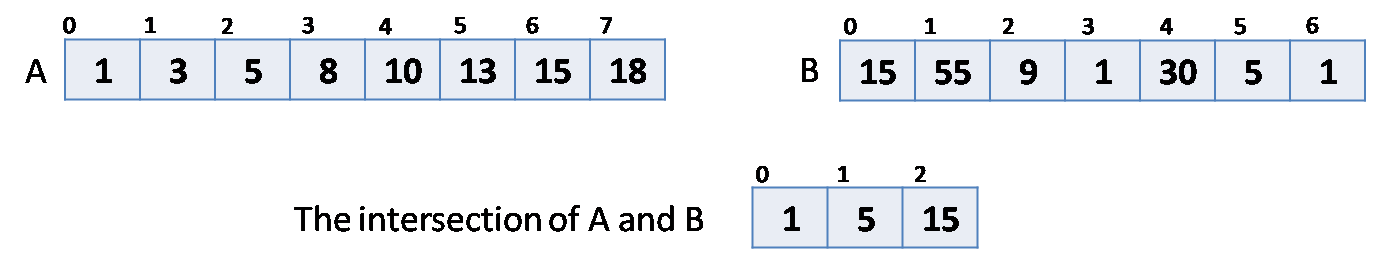
\includegraphics[width=0.7\textwidth]{img/conceptual.png}
\end{center}

\vspace{-1ex}
Unfortunately, we cannot just return the intersection as an array and
expect the client to know how long this array is, so we have to do
something a little bit more fancy --- we have the client give us an
array that they want to be filled with the intersection, and we just
return the number of integers in the intersection. The example above
would now look like this:
\begin{center}
  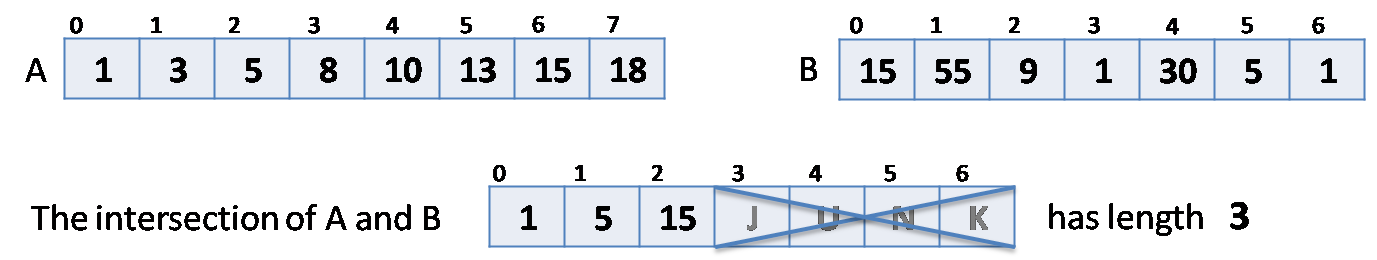
\includegraphics[width=0.7\textwidth]{img/actual.png}
\end{center}
\end{elaboration}

\vspace{-2ex}
Unfortunately, he is busy teaching 122, and so he decided to
offload writing tests to his trusted TAs.  Then he remembered that all
his TAs are busy as well, and came up with the perfect alternative:
have \emph{students} write the tests so he can see who
would be a good TA! A truly ingenious solution!
